\documentclass{article}

\usepackage{fancyhdr}
\usepackage{extramarks}
\usepackage{amsmath}
\usepackage{amsthm}
\usepackage{amsfonts}
\usepackage{tikz}
\usepackage[plain]{algorithm}
\usepackage{algpseudocode}
\usepackage{enumerate}
\usepackage{tikz}
\usepackage{graphicx}
\usepackage{subfigure}

%
% Basic Document Settings
%  

\topmargin=-0.45in
\evensidemargin=0in
\oddsidemargin=0in
\textwidth=6.5in
\textheight=9.0in
\headsep=0.25in

\linespread{1.1}

\pagestyle{fancy}


\renewcommand\headrulewidth{0.4pt}
\renewcommand\footrulewidth{0.4pt}

\setlength\parindent{0pt}


%
% Title Page
%

\title{
    \vspace{2in}
    \textmd{\textbf{Report for Electromagnetics Class Projects}}\\
    \vspace{2in}
}

\author{
	Name: \textbf{ZhuYuxuan QuGechen} \\
	Student ID: 2020531016 2020531054}
\date{\today}


\everymath{\displaystyle}
\begin{document}

\maketitle
\pagebreak

\section{Deduction $Z_2$ from $\Gamma,T$}

Firstly, in the coaxial line, there are the following expressions for electric and magnetic fields:
\begin{align*}
    E &=\frac{V\cdot \hat{\rho } }{\rho \cdot \ln(b/a)}\\
    H &=\frac{I\cdot \hat{\phi} }{2\pi\phi}
\end{align*}
Because there is no surface current and surface charge distribution on the interfaces of $z=z_0$ and $z=z_0+d$,
the electric field and magnetic field are continuous on the two interfaces.
Therefore, the voltage and current are continuous on the two interfaces.\\

Contact the voltage and current expressions in the coaxial line, in medium 1 ($z<z_0$)we have
\begin{align*}
    \tilde{V}_1(z) & = V_0^i(e^{-\gamma_1z}+\Gamma e^{\gamma_1z})\\
    \tilde{I}_1(z) & = \frac{V_0^i}{Z_1}(e^{-\gamma_1z}-\Gamma e^{\gamma_1z})
\end{align*}
in medium 2 ($z_0<z<z_0+d$), assume the magnitudes of voltage as $B,C$, it becomes to
\begin{align*}
    \tilde{V}_2(z) & = Be^{-\gamma_2z}+C e^{\gamma_2z}\\
    \tilde{I}_2(z) & = \frac{B}{Z_2}e^{-\gamma_2z}-\frac{C}{Z_2} e^{\gamma_2z}
\end{align*}
in medium 3, it only has transmission wave, then it becomes to
\begin{align*}
    \tilde{V}_3(z) & = Te^{-\gamma_1z}\\
    \tilde{I}_3(z) & = \frac{T}{Z_1}e^{-\gamma_1z}
\end{align*}

Then we have
\begin{align*}
    \tilde{V}_1(z_0) &= \tilde{V}_2(z_0)\\
    \tilde{I}_1(z_0) &= \tilde{I}_2(z_0)\\
    \tilde{V}_2(z_0+d) &= \tilde{V}_3(z_0+d)\\
    \tilde{I}_2(z_0+d) &= \tilde{I}_3(z_0+d)
\end{align*}
Since only the ratio to the incident wave mode value is concerned, we set $V_0^i=1$, then the four equations become to
\begin{align*}
    {\mathrm{e}}^{-\gamma_1 \,z_0 } +\Gamma \,{\mathrm{e}}^{\gamma_1 \,z_0 } =B\,{\mathrm{e}}^{-\gamma_2 \,z_0 } +C\,{\mathrm{e}}^{\gamma_2 \,z_0 }\\
    \frac{{\mathrm{e}}^{-\gamma_1 \,z_0 } -\Gamma \,{\mathrm{e}}^{\gamma_1 \,z_0 } }{Z_1 }=\frac{B\,{\mathrm{e}}^{-\gamma_2 \,z_0 } -C\,{\mathrm{e}}^{\gamma_2 \,z_0 } }{Z_2 }\\
    B\,{\mathrm{e}}^{-\gamma_2 \,{\left(d+z_0 \right)}} +C\,{\mathrm{e}}^{\gamma_2 \,{\left(d+z_0 \right)}} =\mathrm{T}\,{\mathrm{e}}^{-\gamma_1 \,{\left(d+z_0 \right)}}\\
    \frac{B\,{\mathrm{e}}^{-\gamma_2 \,{\left(d+z_0 \right)}} -C\,{\mathrm{e}}^{\gamma_2 \,{\left(d+z_0 \right)}} }{Z_2 }=\frac{\mathrm{T}\,{\mathrm{e}}^{-\gamma_1 \,{\left(d+z_0 \right)}} }{Z_1 }
\end{align*}
Following the turtorial, with the help of matlab, we can use $\Gamma,T$ to express  $Z_2,\gamma_2$
\begin{align*}
    \Gamma &= \left\{\begin{array}{l}
        -\frac{{\mathrm{e}}^{-2\,\gamma_1 \,z_0 } \,{\left(\sigma_2 -\sigma_4 -\sigma_1 +\sigma_3 \right)}}{\sigma_2 -\sigma_4 +\sigma_1 -\sigma_3 +2\,Z_1 \,Z_2 \,{\mathrm{e}}^{\gamma_2 \,{\left(d+z_0 \right)}} \,{\mathrm{e}}^{-\gamma_2 \,z_0 } +2\,Z_1 \,Z_2 \,\sigma_5 \,{\mathrm{e}}^{\gamma_2 \,z_0 } }\\
        \mathrm{}\\
        \textrm{where}\\
        \mathrm{}\\
        \;\;\sigma_1 ={Z_2 }^2 \,{\mathrm{e}}^{\gamma_2 \,{\left(d+z_0 \right)}} \,{\mathrm{e}}^{-\gamma_2 \,z_0 } \\
        \mathrm{}\\
        \;\;\sigma_2 ={Z_1 }^2 \,{\mathrm{e}}^{\gamma_2 \,{\left(d+z_0 \right)}} \,{\mathrm{e}}^{-\gamma_2 \,z_0 } \\
        \mathrm{}\\
        \;\;\sigma_3 ={Z_2 }^2 \,\sigma_5 \,{\mathrm{e}}^{\gamma_2 \,z_0 } \\
        \mathrm{}\\
        \;\;\sigma_4 ={Z_1 }^2 \,\sigma_5 \,{\mathrm{e}}^{\gamma_2 \,z_0 } \\
        \mathrm{}\\
        \;\;\sigma_5 ={\mathrm{e}}^{-\gamma_2 \,{\left(d+z_0 \right)}} 
        \end{array}\right.\\
    T &= \left\{\begin{array}{l}
        \frac{4\,Z_1 \,Z_2 \,{\mathrm{e}}^{\gamma_1 \,{\left(d+z_0 \right)}} \,{\mathrm{e}}^{-\gamma_1 \,z_0 } }{{Z_1 }^2 \,\sigma_2 \,{\mathrm{e}}^{-\gamma_2 \,z_0 } -{Z_1 }^2 \,\sigma_1 \,{\mathrm{e}}^{\gamma_2 \,z_0 } +{Z_2 }^2 \,\sigma_2 \,{\mathrm{e}}^{-\gamma_2 \,z_0 } -{Z_2 }^2 \,\sigma_1 \,{\mathrm{e}}^{\gamma_2 \,z_0 } +2\,Z_1 \,Z_2 \,\sigma_2 \,{\mathrm{e}}^{-\gamma_2 \,z_0 } +2\,Z_1 \,Z_2 \,\sigma_1 \,{\mathrm{e}}^{\gamma_2 \,z_0 } }\\
        \mathrm{}\\
        \textrm{where}\\
        \mathrm{}\\
        \;\;\sigma_1 ={\mathrm{e}}^{-\gamma_2 \,{\left(d+z_0 \right)}} \\
        \mathrm{}\\
        \;\;\sigma_2 ={\mathrm{e}}^{\gamma_2 \,{\left(d+z_0 \right)}} 
        \end{array}\right.
\end{align*}
Based on that, we can find out the expression of $Z_2,\gamma_2$ using $\Gamma,T$, that is
\begin{align*}
    Z_2 = \left\{\begin{array}{l}
        \left(\begin{array}{c}
        \frac{Z_1 \,{\left(\sigma_6 +{\mathrm{T}}^2 \,{\mathrm{e}}^{2\,\gamma_1 \,z_0 } +\sigma_1 -\Gamma^2 \,\sigma_6 \,{\mathrm{e}}^{4\,\gamma_1 \,z_0 } \right)}}{\sigma_4 }-\sigma_2 \\
        \frac{Z_1 \,{\left(\sigma_6 +{\mathrm{T}}^2 \,{\mathrm{e}}^{2\,\gamma_1 \,z_0 } -\sigma_1 -\Gamma^2 \,\sigma_6 \,{\mathrm{e}}^{4\,\gamma_1 \,z_0 } \right)}}{\sigma_4 }-\sigma_2 
        \end{array}\right)\\
        \mathrm{}\\
        \textrm{where}\\
        \mathrm{}\\
        \;\;\sigma_1 =\sqrt{-{\left(\mathrm{T}\,{\mathrm{e}}^{\gamma_1 \,z_0 } -\sigma_5 +\sigma_3 \right)}\,{\left(\sigma_5 +\mathrm{T}\,{\mathrm{e}}^{\gamma_1 \,z_0 } +\sigma_3 \right)}\,{\left(\sigma_5 +\mathrm{T}\,{\mathrm{e}}^{\gamma_1 \,z_0 } -\sigma_3 \right)}\,{\left(\sigma_5 -\mathrm{T}\,{\mathrm{e}}^{\gamma_1 \,z_0 } +\sigma_3 \right)}}\\
        \mathrm{}\\
        \;\;\sigma_2 =\frac{Z_1 \,{\left(-\sigma_6 \,{\mathrm{e}}^{4\,\gamma_1 \,z_0 } \,\Gamma^2 +{\mathrm{e}}^{2\,\gamma_1 \,z_0 } \,{\mathrm{T}}^2 +\sigma_6 \right)}}{\sigma_4 }\\
        \mathrm{}\\
        \;\;\sigma_3 =\Gamma \,\sigma_5 \,{\mathrm{e}}^{2\,\gamma_1 \,z_0 } \\
        \mathrm{}\\
        \;\;\sigma_4 =\sigma_6 \,{\mathrm{e}}^{4\,\gamma_1 \,z_0 } \,\Gamma^2 -2\,\sigma_6 \,{\mathrm{e}}^{2\,\gamma_1 \,z_0 } \,\Gamma -{\mathrm{e}}^{2\,\gamma_1 \,z_0 } \,{\mathrm{T}}^2 +\sigma_6 \\
        \mathrm{}\\
        \;\;\sigma_5 ={\mathrm{e}}^{\gamma_1 \,{\left(d+z_0 \right)}} \\
        \mathrm{}\\
        \;\;\sigma_6 ={\mathrm{e}}^{2\,\gamma_1 \,{\left(d+z_0 \right)}} 
        \end{array}\right.\\
\end{align*}
\begin{align*}
    \gamma_2 = \left\{\begin{array}{l}
        \left(\begin{array}{c}
        \frac{\log \left(\frac{{\mathrm{e}}^{-\gamma_1 \,{\left(d+z_0 \right)}} \,{\mathrm{e}}^{-\gamma_1 \,z_0 } \,{\left(\sigma_5 +{\mathrm{T}}^2 \,{\mathrm{e}}^{2\,\gamma_1 \,z_0 } +\sigma_1 -\sigma_2 \right)}}{2\,\mathrm{T}}\right)}{d}\\
        \frac{\log \left(\frac{{\mathrm{e}}^{-\gamma_1 \,{\left(d+z_0 \right)}} \,{\mathrm{e}}^{-\gamma_1 \,z_0 } \,{\left(\sigma_5 +{\mathrm{T}}^2 \,{\mathrm{e}}^{2\,\gamma_1 \,z_0 } -\sigma_1 -\sigma_2 \right)}}{2\,\mathrm{T}}\right)}{d}
        \end{array}\right)\\
        \mathrm{}\\
        \textrm{where}\\
        \mathrm{}\\
        \;\;\sigma_1 =\sqrt{-{\left(\sigma_4 -\sigma_6 +\sigma_3 \right)}\,{\left(\sigma_6 +\sigma_4 +\sigma_3 \right)}\,{\left(\sigma_6 +\sigma_4 -\sigma_3 \right)}\,{\left(\sigma_6 -\sigma_4 +\sigma_3 \right)}}\\
        \mathrm{}\\
        \;\;\sigma_2 =\Gamma^2 \,\sigma_5 \,{\mathrm{e}}^{4\,\gamma_1 \,z_0 } \\
        \mathrm{}\\
        \;\;\sigma_3 =\Gamma \,\sigma_6 \,{\mathrm{e}}^{2\,\gamma_1 \,z_0 } \\
        \mathrm{}\\
        \;\;\sigma_4 =\mathrm{T}\,{\mathrm{e}}^{\gamma_1 \,z_0 } \\
        \mathrm{}\\
        \;\;\sigma_5 ={\mathrm{e}}^{2\,\gamma_1 \,{\left(d+z_0 \right)}} \\
        \mathrm{}\\
        \;\;\sigma_6 ={\mathrm{e}}^{\gamma_1 \,{\left(d+z_0 \right)}} 
        \end{array}\right.
\end{align*}

\section{Deduction other parameters}
From the lots, we have
\begin{align*}
    a &= 0.002m\\
    b &= 0.003m\\
    d &= 0.55m\\
    \epsilon_1 &= 1\\
    f &= 10^9Hz\\
\end{align*}
Then we have
\begin{align*}
    \gamma_1 &= j*\omega*\sqrt{\mu_0\epsilon_1\epsilon_0}\\
    Z_1 &= \frac{60\ln(b/a)}{\sqrt{\epsilon_1\epsilon_0}}
\end{align*}
Due to the property of coaxial lines, we have
\begin{align*}
    Z = \frac{60\ln(b/a)}{\sqrt{\epsilon}}
\end{align*}
where $\epsilon$ can be the complex permitivity. Therefore we have
\begin{align*}
    \epsilon_2 = \frac{\mu_0}{Z_2^2(2\pi/\ln(b/a))^2}
\end{align*}

\section{Calculation and Simulation 1}
With the first group of coefficients, we have
\begin{align*}
    \Gamma_1 &= -0.18367707842865-0.336458601842074i\\
    T_1 &= -0.73358668120551-0.561167203468699i
\end{align*}

\begin{align*}
    Z_2 &=     8.103846546579724 - 0.000090357978102i\ \Omega \\
    \gamma_2 &=  0.000049836674385 -51.364551044460249i\ m^{-1}
\end{align*}
Actually, there are two solutions for $Z_2$ and $\gamma_2$, however, the real part of the other solution for $Z_2$ is negative,
which is impossible in real world, so we discard that solution.\\

Then by further calculating, we have
\begin{align*}
    \epsilon_2 &=  7.968465274556406*10^{-11} + 1.776969508829155*10^{-15}i\\
    \epsilon_{r2} &= \frac{real(\epsilon_2)}{\epsilon_0}\approx 8.999656929862034\\
    \sigma &= -imag(\epsilon_2)*\omega \approx -1.116502870918147*10^{-5} \approx 0 S/m
\end{align*}

Set the length of medium 1 of both two sides as $d_2 = \lambda_1$, which allows us ignore the phase difference caused by medium 1,
then we have the following model\\
\begin{figure}[h]
    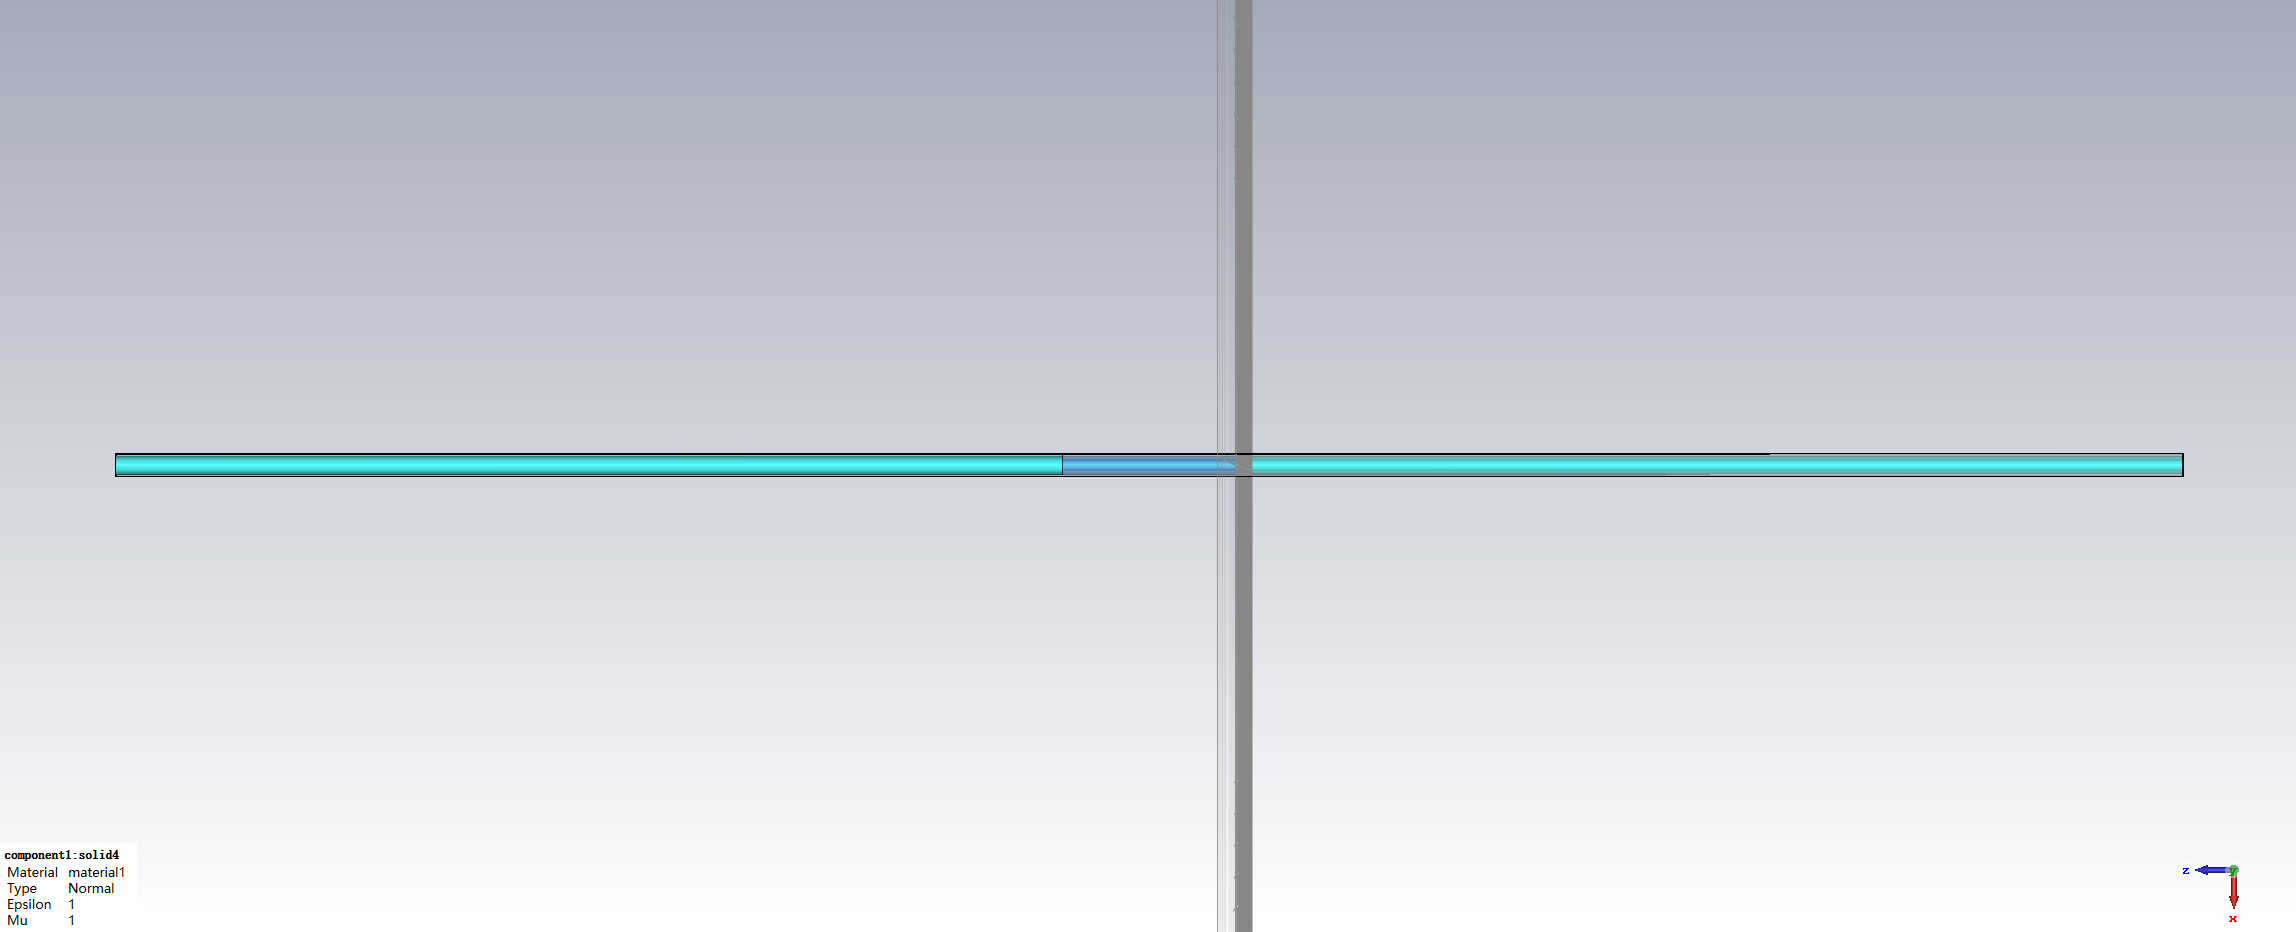
\includegraphics[width=1\textwidth]{1.png}
\end{figure}

\pagebreak
By simulation, we have
\begin{figure}[h]
    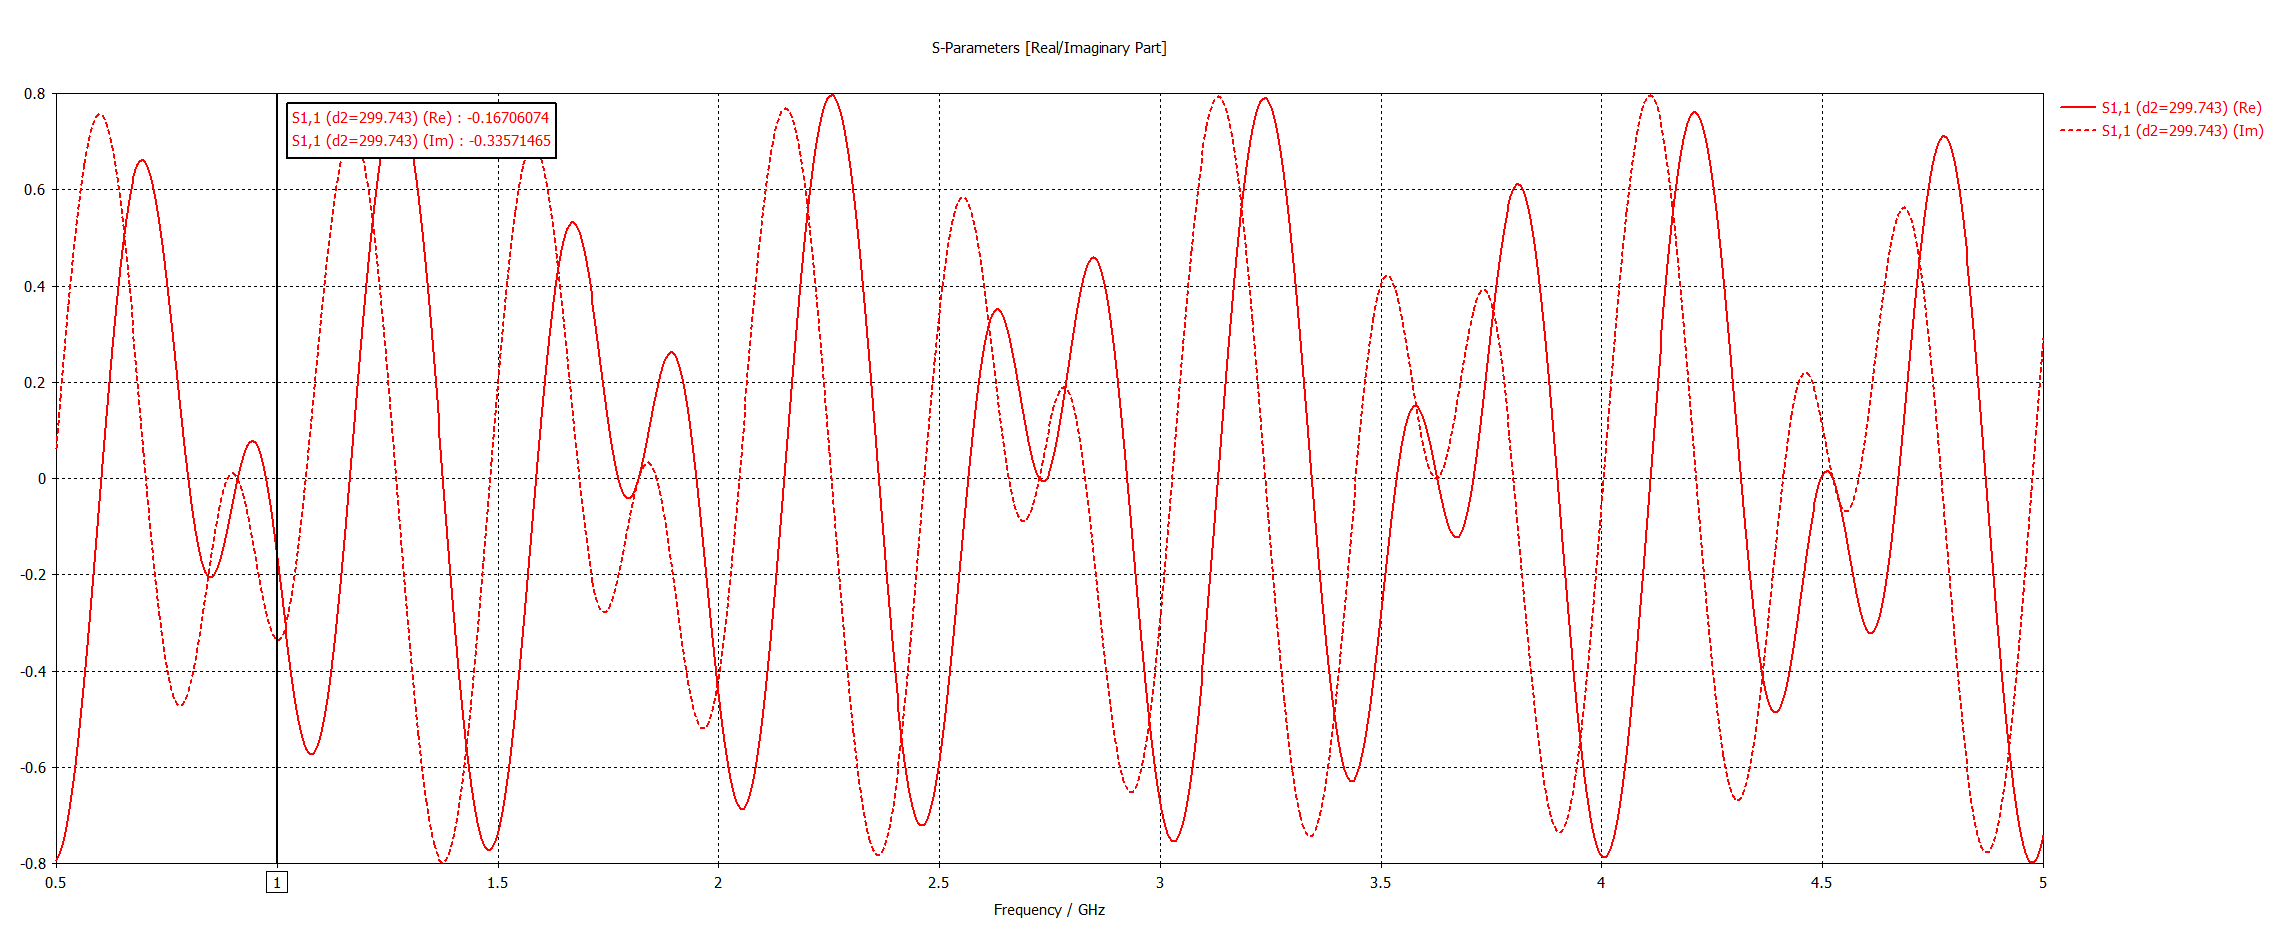
\includegraphics[width=1\textwidth]{2.png}
    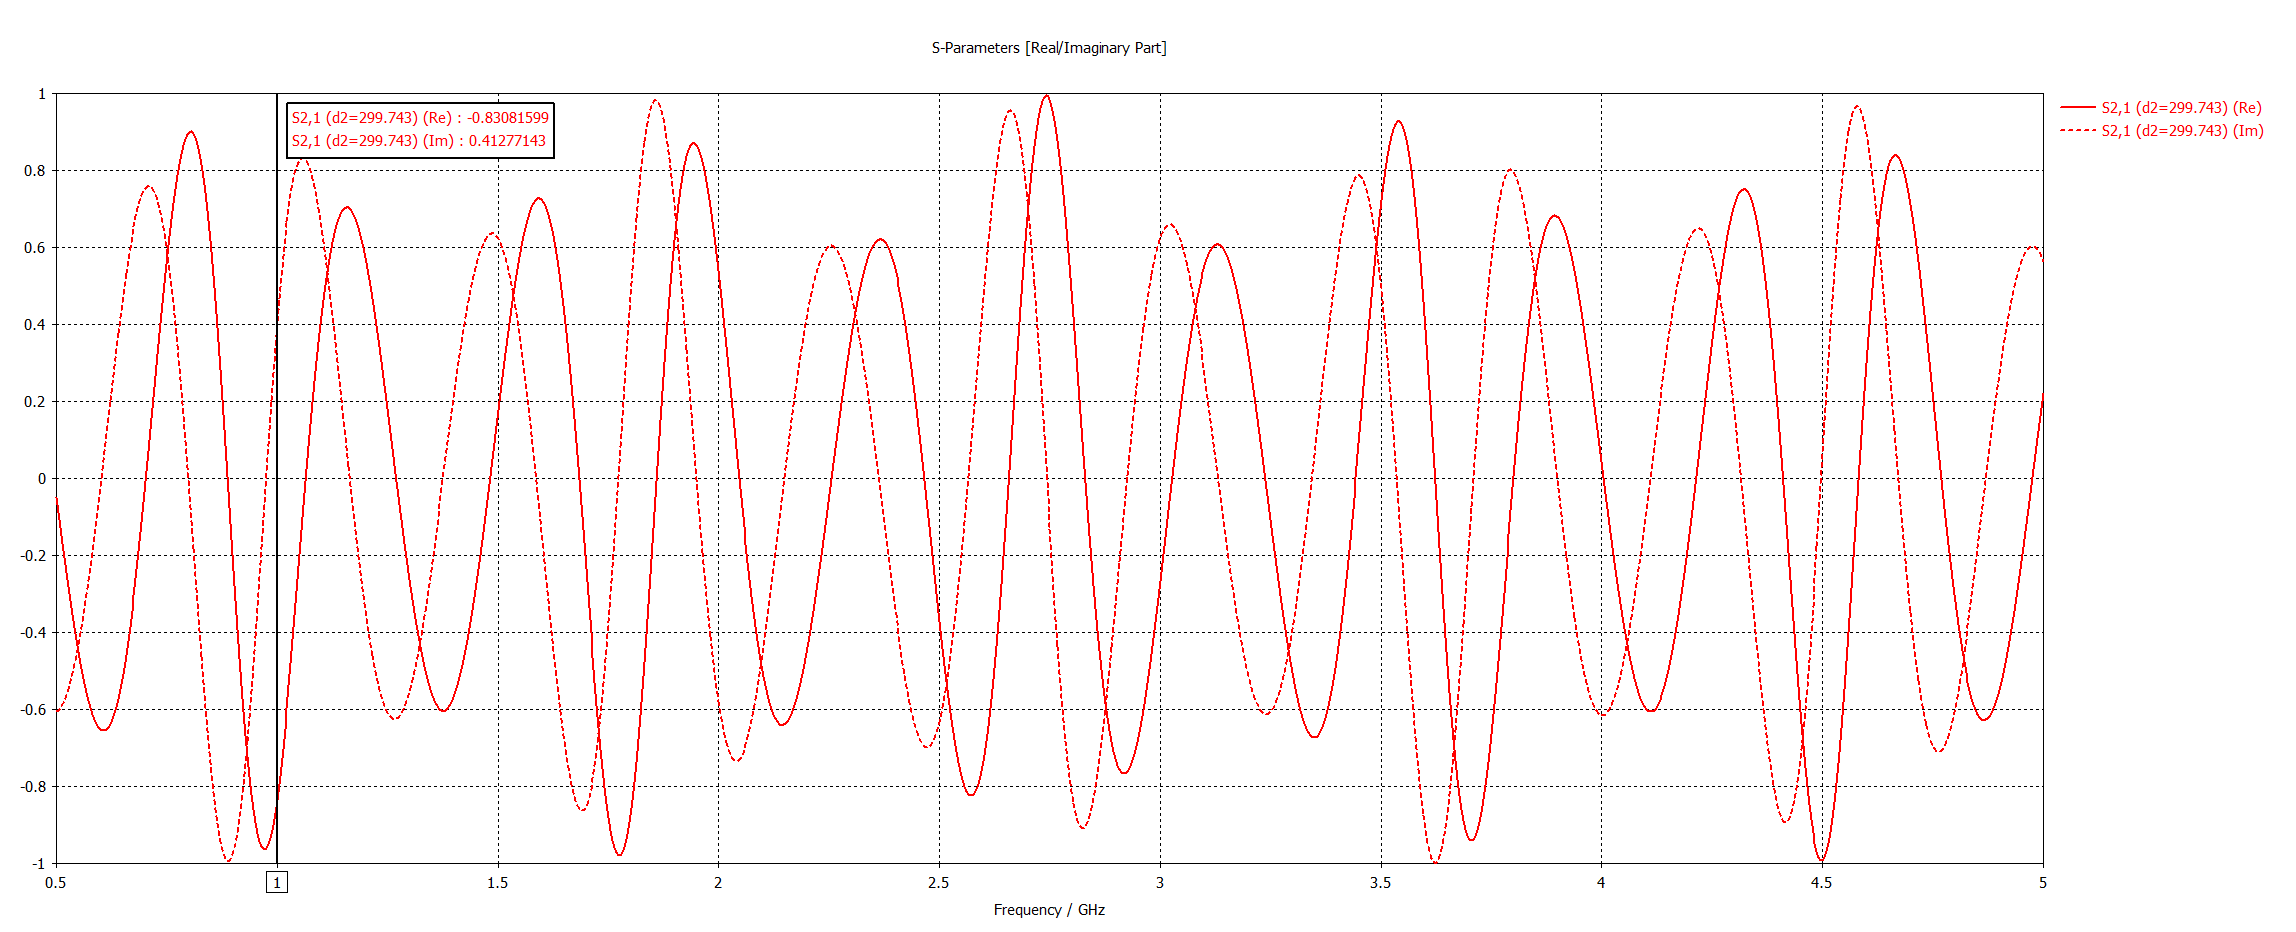
\includegraphics[width=1\textwidth]{3.png}
\end{figure}
thus we obtain
\begin{align*}
    S_{11} & = -0.16706074-0.33571465i \approx \Gamma_1\\
    S_{21} &= T_1 = -0.83081599+0.41277143i\\
    &\approx T1*e^{-\gamma_1d} = -0.810675666421054 + 0.442564134294426i
\end{align*}
which is within the allowable error range.

\section{Calculation and Simulation 2}
With the second group of coefficients, we have
\begin{align*}
    \Gamma_2 &= -0.195677924334674+0.116950135912389i\\
    T_2 &= -0.134265494843727-0.7238751863504i
\end{align*}
However, the $T$ we assumed in the equation is $\frac{\tilde{V}^r(z_0+d)}{\tilde{V}^i(z_0)}$,
therefore, we should use $T_1\cdot e^{-\gamma_1 d}$ instead of $T_1$ to solve $\epsilon_2$.

\begin{align*}
    Z_2 &=   9.384395457555984 + 0.700022010466726i\ \Omega \\
    \gamma_2 &= -4.026968258633184 -53.993480480585660i\ m^{-1}
\end{align*}
Actually, there are two solutions for $Z_2$ and $\gamma_2$, however, the real part of the other solution for $Z_2$ is negative,
which is impossible in real world, so we discard that solution.\\

Then by further calculating, we have
\begin{align*}
    \epsilon_2 &=  5.843882975868956*10^{-11} - 8.767185499046495*10^{-12}i\\
    \epsilon_{r2} &= \frac{real(\epsilon_2)}{\epsilon_0}\approx    6.600134418482435\\
    \sigma &= -imag(\epsilon_2)*\omega \approx 0.055085851112927
\end{align*}

By simulation, we have
\begin{figure}[h]
    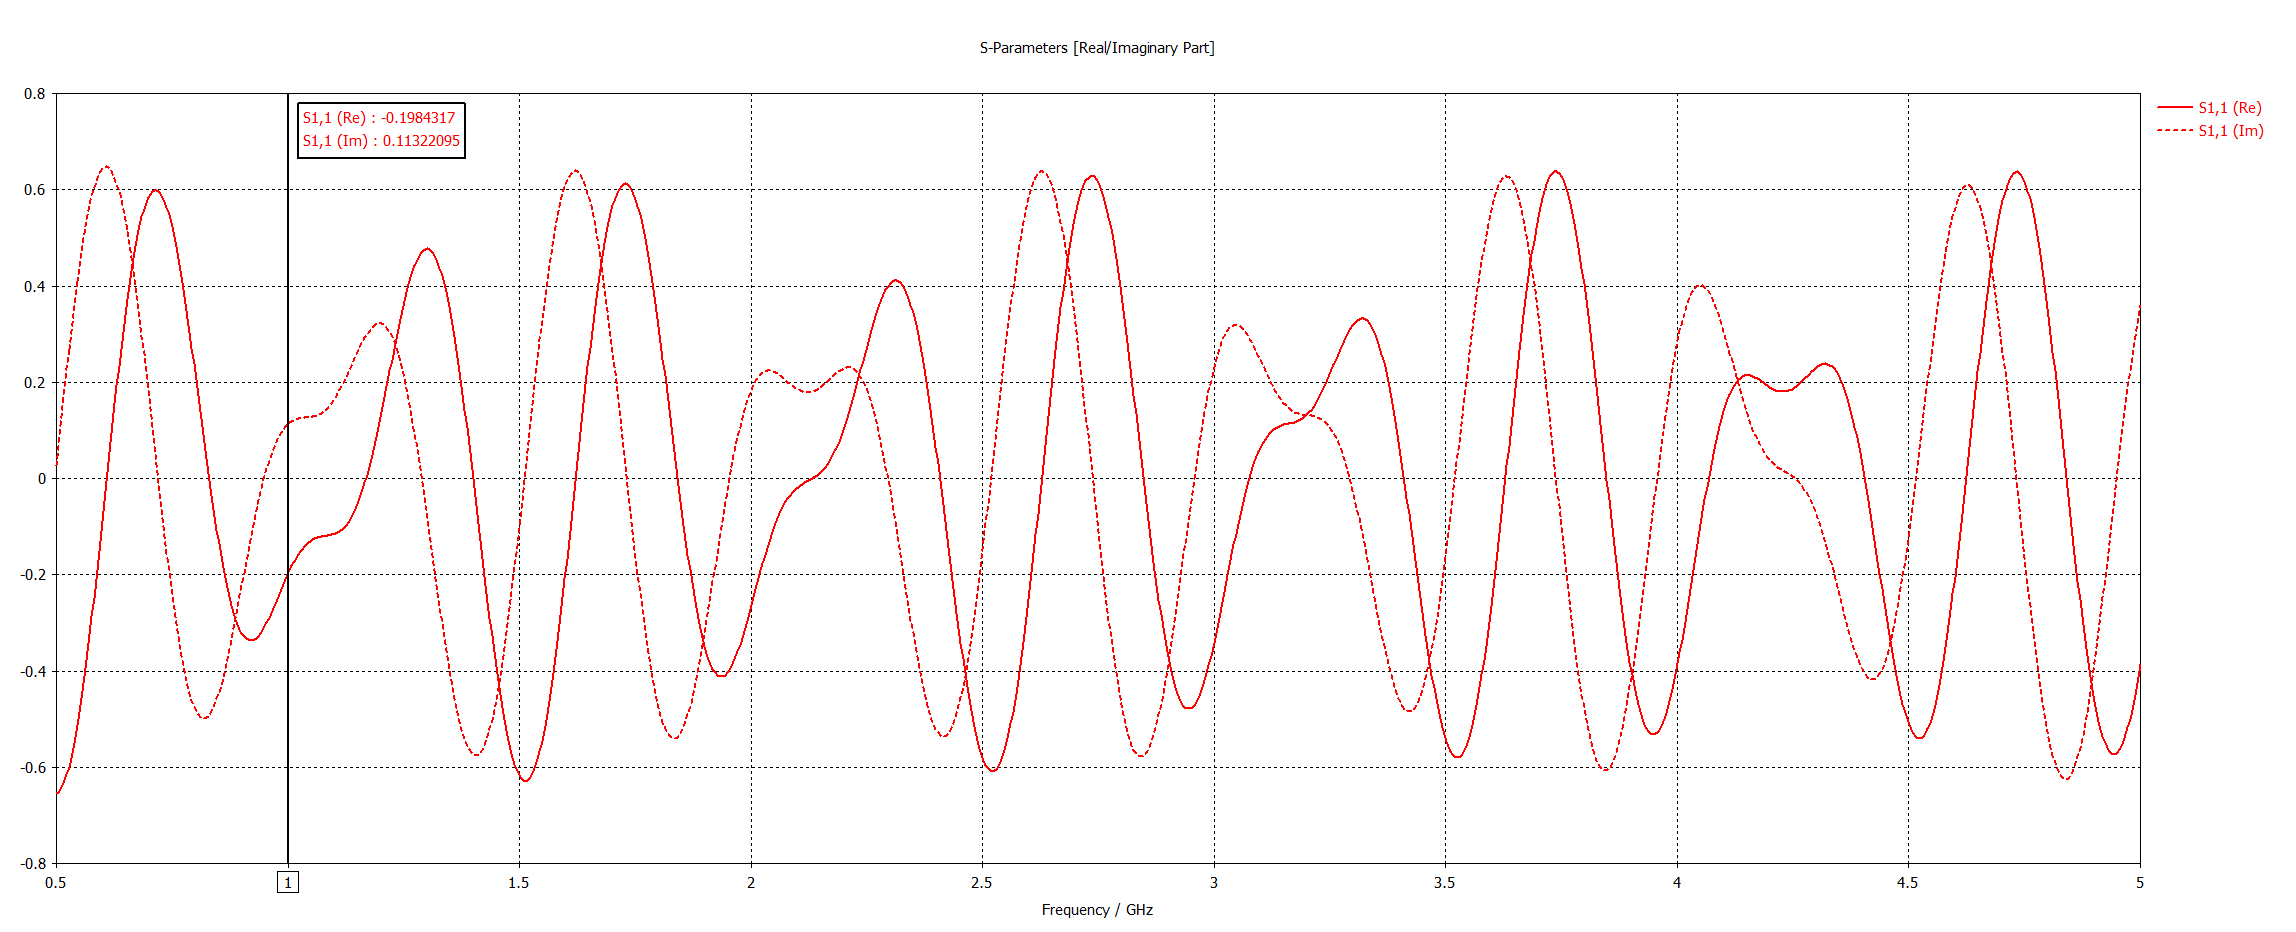
\includegraphics[width=1\textwidth]{4.png}
    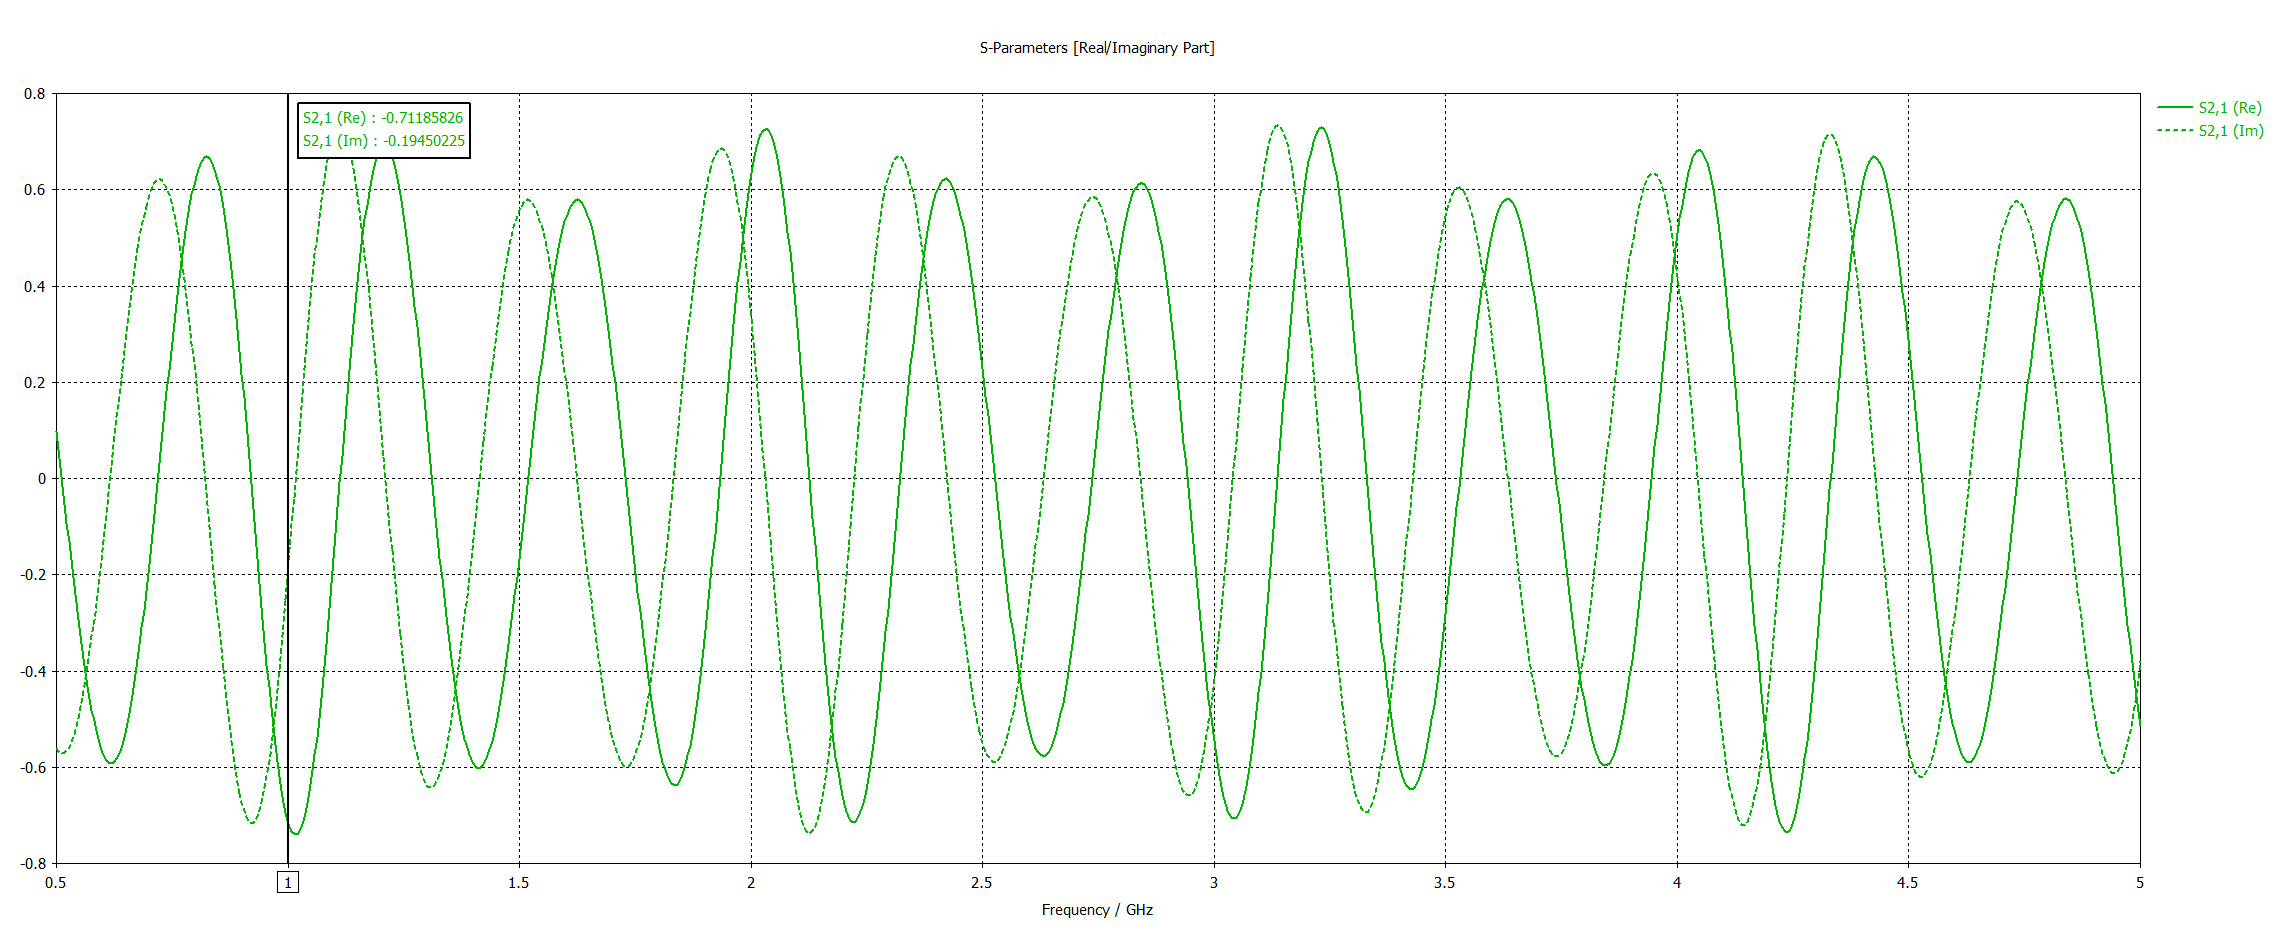
\includegraphics[width=1\textwidth]{5.png}
\end{figure}
thus we obtain
\begin{align*}
    S_{11} & = -0.1984317+0.11322095i \approx \Gamma_2\\
    S_{21} & = -0.71185826-0.19450225i\\
    &\approx T2*e^{-\gamma_1d} = -0.716040335476707 - 0.171197974549531i
\end{align*}
which is within the allowable error range.

\end{document}
